%% 
%% Copyright 2007, 2008, 2009 Elsevier Ltd
%% 
%% This file is part of the 'Elsarticle Bundle'.
%% ---------------------------------------------
%% 
%% It may be distributed under the conditions of the LaTeX Project Public
%% License, either version 1.2 of this license or (at your option) any
%% later version.  The latest version of this license is in
%%    http://www.latex-project.org/lppl.txt
%% and version 1.2 or later is part of all distributions of LaTeX
%% version 1999/12/01 or later.
%% 
%% The list of all files belonging to the 'Elsarticle Bundle' is
%% given in the file `manifest.txt'.
%% 
%% Template article for Elsevier's document class `elsarticle'
%% with harvard style bibliographic references
%% SP 2008/03/01

%\documentclass[preprint,12pt,authoryear]{elsarticle}  %default in the template
%\documentclass[preprint,10pt,authoryear]{elsarticle}

%% Use the option review to obtain double line spacing
%% \documentclass[authoryear,preprint,review,12pt]{elsarticle}

%% Use the options 1p,twocolumn; 3p; 3p,twocolumn; 5p; or 5p,twocolumn
%% for a journal layout:
%% \documentclass[final,1p,times,authoryear]{elsarticle}
%% \documentclass[final,1p,times,twocolumn,authoryear]{elsarticle}
 \documentclass[final,3p,times,authoryear]{elsarticle}
%% \documentclass[final,3p,times,twocolumn,authoryear]{elsarticle}
%% \documentclass[final,5p,times,authoryear]{elsarticle}
%% \documentclass[final,5p,times,twocolumn,authoryear]{elsarticle}

%% For including figures, graphicx.sty has been loaded in
%% elsarticle.cls. If you prefer to use the old commands
%% please give \usepackage{epsfig}

%% The amssymb package provides various useful mathematical symbols
\usepackage{amssymb}
%% The amsthm package provides extended theorem environments
 \usepackage{amsthm}
 \usepackage{amsmath}
 \usepackage{color}
 \usepackage{amsmath}
\usepackage{siunitx}
\usepackage{todonotes}

\usepackage{framed} % Framing content
\usepackage{multicol} % Multiple columns environment
\usepackage{nomencl} % Nomenclature package
\makenomenclature
%\setlength{\nomitemsep}{-\parskip} % Baseline skip between items
\setlength{\nomitemsep}{0.01cm}
\renewcommand*\nompreamble{\begin{multicols}{2}}
\renewcommand*\nompostamble{\end{multicols}}
\newcommand{\degreeC}{\ensuremath{^\circ}C }

%\usepackage[nonumberlist]{glossaries}
%\makeglossaries 


%% The lineno packages adds line numbers. Start line numbering with
%% \begin{linenumbers}, end it with \end{linenumbers}. Or switch it on
%% for the whole article with \linenumbers.
%% \usepackage{lineno}

\journal{Urban Climate}


\begin{document}


%\include{TargetHtc_glossary} 


\begin{frontmatter}

%% Title, authors and addresses

%% use the tnoteref command within \title for footnotes;
%% use the tnotetext command for theassociated footnote;
%% use the fnref command within \author or \address for footnotes;
%% use the fntext command for theassociated footnote;
%% use the corref command within \author for corresponding author footnotes;
%% use the cortext command for theassociated footnote;
%% use the ead command for the email address,
%% and the form \ead[url] for the home page:
%% \title{Title\tnoteref{label1}}
%% \tnotetext[label1]{}
%% \author{Name\corref{cor1}\fnref{label2}}
%% \ead{email address}
%% \ead[url]{home page}
%% \fntext[label2]{}
%% \cortext[cor1]{}
%% \address{Address\fnref{label3}}
%% \fntext[label3]{}

\title{Sky pixel detection in imagery using an adaptive algorithm and machine learning.}


%% use optional labels to link authors explicitly to addresses:


\author[melb]{Kerry~A.~Nice\corref{cor1}}
\ead{kerry.nice@unimelb.edu.au}
\author[melb]{Jasper S. Wijnands}
\author[asu]{Ariane Middel}
\author[cis]{Jingcheng Wang}
\author[cis]{Yiming Qiu}
\author[cis]{Nan Zhao}
\author[melb,sunshine]{Jason Thompson}
\author[melb]{Gideon D.P.A. Aschwanden}
\author[melb]{Haifeng Zhao}
\author[melb,eng]{Mark Stevenson}

\cortext[cor1]{Principal corresponding author}
\address[melb]{Transport, Health, and Urban Design Hub, Faculty of Architecture, Building, and Planning, University of Melbourne, Victoria 3010, Australia}
\address[cis]{School of Computing and Information Systems, University of Melbourne, Victoria 3010, Australia}
\address[eng]{Melbourne School of Engineering; and Melbourne School of Population and Global Health, University of Melbourne, Victoria, Australia.}
\address[sunshine]{Centre for Human Factors and Sociotechnical Systems, University of the Sunshine Coast, Australia.}
%\address[monash]{School of Earth, Atmosphere and Environment, Monash University, Clayton, VIC 3800, Australia}
%\address[az1]{School of Geographical Sciences and Urban Planning, Arizona State University, Tempe, Arizona, USA}
%\address[az2]{Urban Climate Research Center, Arizona State University, Tempe, Arizona, USA}
%\address[crc]{Cooperative Research Centre for Water Sensitive Cities, Melbourne, Australia}
\address[asu]{School of Computing, Informatics, and Decision Systems Engineering (CIDSE), Arizona State University}





\begin{abstract}

%Urban heat is a significant health risk, especially during extreme heat days. Identifying vulnerable areas of cities is a priority for devising effective heat mitigation strategies. However, making these observations is difficult, expensive, and time consuming. The platform developed through this project allows systematic assessments to be made for any urban area using a global and consistent dataset, Google Street View (GSV) imagery. The imagery is processed using an ensemble of OpenCV mean-shift segmentation, K-means clustering, and HSL based colour filtering to mark sky pixels in the image and extract sky view factors (SVF). The images are pre-classified prior to clustering by a convolutional neural network (CNN), trained with 40,000 images from the Skyfinder dataset \citep{Mihail2016}. This pre-classification step allows the sky marking to follow an adaptive process and to use different techniques and parameters based on the content of the images (i.e. tall buildings, clear sky, cloudy sky, tree-filled sky, etc.). The same imagery and processing techniques are also used to find a green-view index (amount of visible vegetation) and a breakdown of urban surface fractions for each scene, which are then individually modelled using the VTUF-3D and TARGET models to assess mean radiant temperatures and human thermal comfort (HTC) indexes. 

%The resulting platform advances the knowledge base in a number of research areas. It will facilitate research into urban green spaces and assist with understanding the impact of urban design on human health. This method allows collection of urban parameters, enabling more detailed and accurate urban modelling domains to be designed. Finally, in the urban design area, these techniques allow urban areas to be quickly scanned for their thermal performance under a variety of weather conditions and allows a determination of the health impacts on city-dwellers and to identify vulnerable areas, areas that should be prioritised for remediation.



\end{abstract}

\begin{keyword}
 
%% keywords here, in the form: keyword \sep keyword

%% PACS codes here, in the form: \PACS code \sep code

%% MSC codes here, in the form: \MSC code \sep code
%% or \MSC[2008] code \sep code (2000 is the default)

\end{keyword}

\end{frontmatter}







\section{Introduction}\label{sec:introduction}

Sky segmentation is a surprisingly difficult computer vision problem. 

Lots of people have tried it. Here's how they tried to do it.

Sky detection is the first step in calculating SVF from images. Once the sky is marked, fisheyes then SVF.

SVF is useful for lots of things.

Here's a system to accurately mark the sky using any type of imagery. Will be demonstrated using Skyfinder images and hand marked GSV images.


\subsection{Research aims}





\section{Methods}\label{sec:Methods}

The sky segmentation in this platform is based on three different computer vision techniques, mean shift and K-means clustering, and a hybrid probability model based on Sobel operators. Using these three techniques, a total of 13 different combinations of techniques and parameters were used, as detailed in Table \ref{tab:techniques}.




\subsection{Skyfinder data}\label{sec:finderdata}
To train the neural network and evaluate the results, images from the Skyfinder dataset \citep{Mihail2016} were used. This dataset was built from 90,000 long-term timelapse images from 53 outdoor webcams over a variety of lighting and weather conditions. Images are of a wide range of sizes and aspect ratios, including 640x489, 857x665, 960x600, 1280x720, and 1280x960. For each location, a binary sky mask was created for validation purposes. In this study, we selected 38,115 images from 40 locations, removing night-time and images with heavy fog as these conditions are unlikely to be encountered in imagery used to calculate sky view factor (i.e. Google Street View).

\subsection{GSV data}\label{sec:gsvdata}
Panoramas for 407 locations in a variety of cities (Adelaide, Brisbane, Paris, Sydney, Tokyo, Perth, and Melbourne) were retrieved using the Google Maps API \citep{GoogleMaps2017b}. Sky pixels in validation images were hand marked for each.

\subsection{Techniques}
14 different technique variations were tested in this project. They are listed in Table \ref{tab:techniques}.

\begin{table}[!htbp]
\caption{\bf Techniques and parameter variations used for sky pixel detection.  \label{tab:techniques}}     
\begin{tabular}{ l  l l}
\textbf{Abbreviation} & \textbf{Section} & \textbf{Technique}  \\ \hline
Mean\_7\_8\_300 & \ref{sec:mean} & Mean shift \\
Mean\_3\_6\_100	 & \ref{sec:mean} & Mean shift \\
Mean\_5\_7\_210	 & \ref{sec:mean} & Mean shift \\	 
Mean\_7\_6\_100	 & \ref{sec:mean} & Mean shift \\
K-mean\_12 & \ref{sec:kmeans} & K-means clustering and HSL color filtering \\
K-mean\_6 & \ref{sec:kmeans} &  K-means clustering and HSL color filtering \\
K-mean\_14 & \ref{sec:kmeans} & K-means clustering and HSL color filtering \\
Sobel\_50 & \ref{sec:prob} & Sobel operator/hybrid probability model \\	  
Sobel\_60 & \ref{sec:prob} & Sobel operator/hybrid probability model \\	
Sobel\_70 & \ref{sec:prob} & Sobel operator/hybrid probability model \\	
Sobel\_80 & \ref{sec:prob} & Sobel operator/hybrid probability model\\
Sobel\_90 & \ref{sec:prob} & Sobel operator/hybrid probability model \\
Sobel\_95 & \ref{sec:prob} & Sobel operator/hybrid probability model \\
Floodfill & \ref{sec:floodfill} & Sobel operator/flood-fill \\
\hline
\end{tabular}
\end{table}


\begin{table}[!htbp]
\caption{\bf Mean shift parameters \label{tab:techniques2}}     
\begin{tabular}{ l  l  l l}
\textbf{Abbreviation}  & \textbf{Spatial radius}&\textbf{Range radius}&\textbf{Min. density}   \\ \hline
Mean\_7\_8\_300 & 7 & 8& 300 \\
Mean\_3\_6\_100	 & 3& 6& 100 \\
Mean\_5\_7\_210	 & 5& 7& 210 \\	 
Mean\_7\_6\_100	 & 7& 6& 100 \\

\hline
\end{tabular}
\end{table}

\begin{table}[!htbp]
\caption{\bf K-means parameters  \label{tab:techniques3}}     
\begin{tabular}{ l l l l l l l l}
\textbf{Abbreviation} & \textbf{Clusters} & \textbf{Skyreq}&\textbf{H uplimit}&\textbf{H downlimit} & \textbf{L lightness} & \textbf{L gray}& \textbf{S gray} \\ \hline
K-mean\_12  & 12 & 0.7& 0.75& 0.3 & 0.95 & 0.75 & 0.2 \\
K-mean\_6  & 6 & 0.6& 0.75& 0.3 & 0.95 & 0.75 & 0.2 \\
K-mean\_14  & 14 & 0.4& 0.75& 0.3 & 0.95 & 0.65 & 0.2 \\
\hline
\end{tabular}
\end{table}

	

\begin{table}[!htbp]
\caption{\bf Sobel techniques  \label{tab:techniques4}}     
\begin{tabular}{ l  l }
\textbf{Abbreviation}  & \textbf{Threshold}    \\ \hline

Sobel\_50 & 50\% \\	  
Sobel\_60 & 60\% \\	
Sobel\_70 & 70\% \\	
Sobel\_80 & 80\% \\
Sobel\_90 & 90\% \\
Sobel\_95 & 95\% \\
\hline
\end{tabular}
\end{table}

\subsection{Hybrid probability model}\label{sec:prob}
An implementation of the sky detection algorithm presented in \cite{Wang2015a} was used in this project using OpenCV \citep{Bradski2000}. This method proceeds by calculating gray scale gradient images using x- and y-directional Sobel operators to estimate sky color. An object function attempts to find the best sky-ground boundary in the gradient image using the covariance matrices of a first calculation of sky and ground regions. Using this best sky boundary, the image is again separated into sky and ground regions and a probability model is created from the center and standard deviations of the colors. A second probability model is created from the gradient values. A third probability model is built based on the vertical position of each pixel (higher more likely to be sky). A final probability model, ranking each pixel's probability that it is sky, is generated by applying close operation on the three probability models. \cite{Wang2015a} did not recommend a probability threshold, so a number of thresholds were tested. The technique designations and thresholds are detailed in Table \ref{tab:techniques2}. Results shown in Figure \ref{fig:sobolresults}.



\begin{figure}
\centering    
a)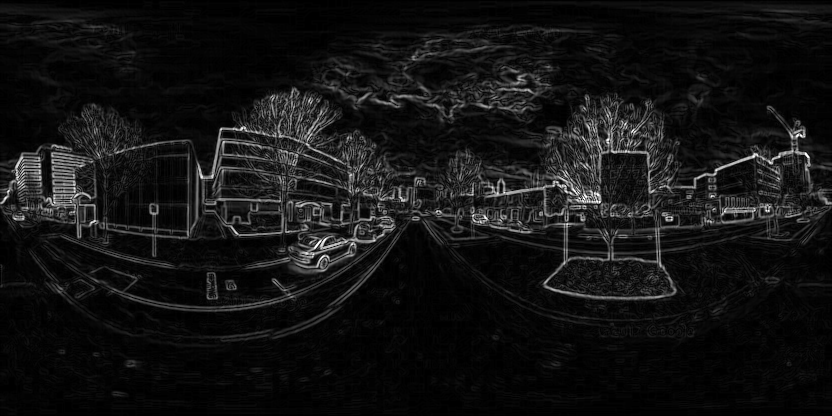
\includegraphics[scale=0.20]{/home/kerryn/git/2018-03-MasterITProject/SkyViewDetection/SkyfinderEvaluationOutput/GSV/mark_output_Sobel/panorama-ESuX4xmQ_fDc50NK6CnfZQ-1_Sobel.png} 
b)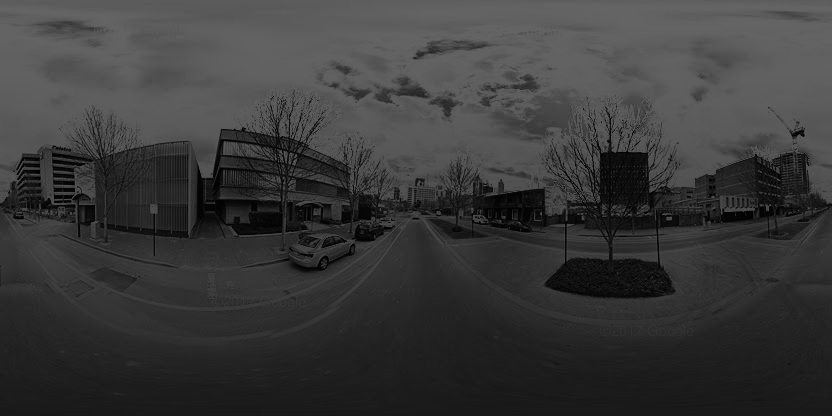
\includegraphics[scale=0.20]{/home/kerryn/git/2018-03-MasterITProject/SkyViewDetection/SkyfinderEvaluationOutput/GSV/mark_output_Sobel/panorama-ESuX4xmQ_fDc50NK6CnfZQ-1_Sobel_prob.png} 
c)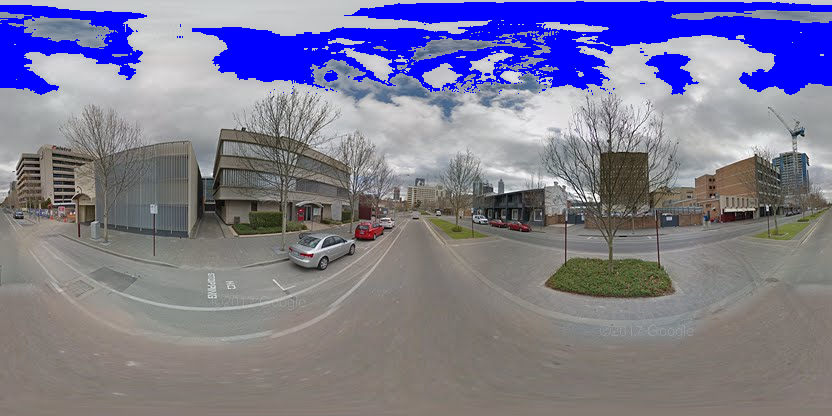
\includegraphics[scale=0.20]{/home/kerryn/git/2018-03-MasterITProject/SkyViewDetection/SkyfinderEvaluationOutput/GSV/mark_output_Sobel/panorama-ESuX4xmQ_fDc50NK6CnfZQ-1_Sobel_95_marked.png} 
d)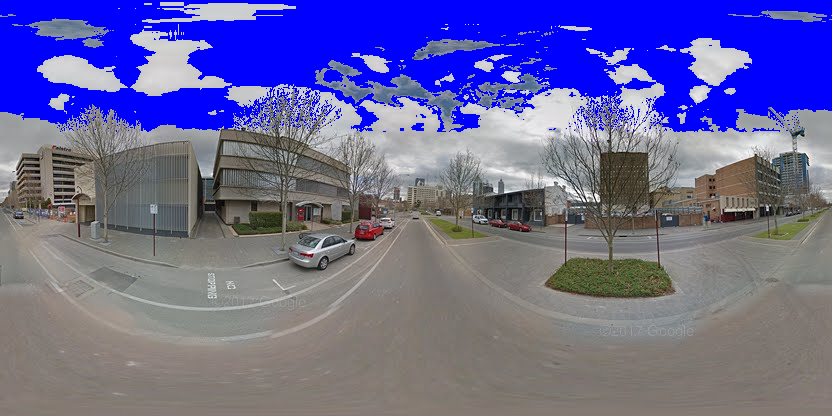
\includegraphics[scale=0.20]{/home/kerryn/git/2018-03-MasterITProject/SkyViewDetection/SkyfinderEvaluationOutput/GSV/mark_output_Sobel/panorama-ESuX4xmQ_fDc50NK6CnfZQ-1_Sobel_90_marked.png} 
e)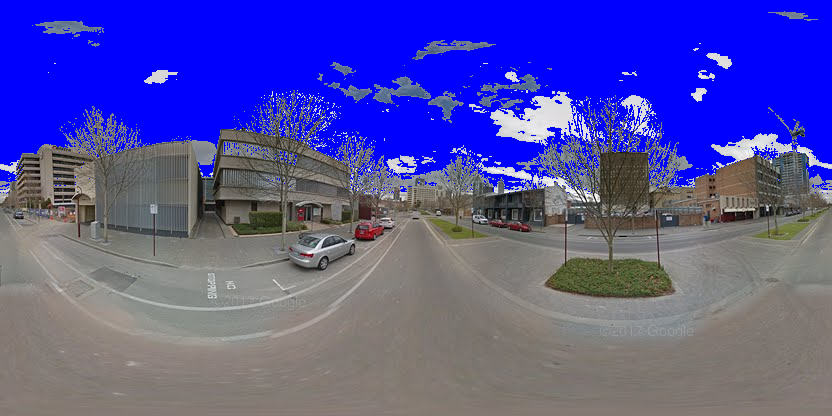
\includegraphics[scale=0.20]{/home/kerryn/git/2018-03-MasterITProject/SkyViewDetection/SkyfinderEvaluationOutput/GSV/mark_output_Sobel/panorama-ESuX4xmQ_fDc50NK6CnfZQ-1_Sobel_80_marked.png} 
f)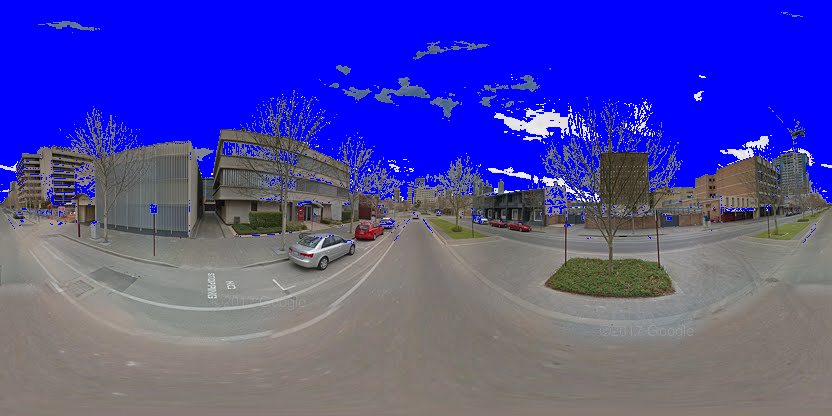
\includegraphics[scale=0.20]{/home/kerryn/git/2018-03-MasterITProject/SkyViewDetection/SkyfinderEvaluationOutput/GSV/mark_output_Sobel/panorama-ESuX4xmQ_fDc50NK6CnfZQ-1_Sobel_70_marked.png} 
g)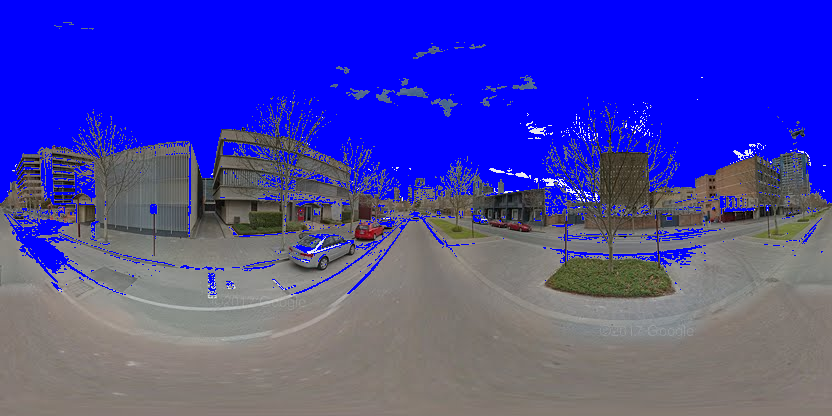
\includegraphics[scale=0.20]{/home/kerryn/git/2018-03-MasterITProject/SkyViewDetection/SkyfinderEvaluationOutput/GSV/mark_output_Sobel/panorama-ESuX4xmQ_fDc50NK6CnfZQ-1_Sobel_60_marked.png} 
h)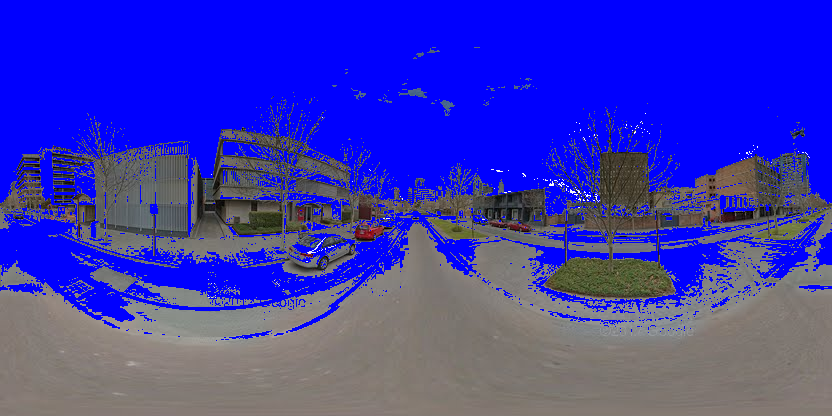
\includegraphics[scale=0.20]{/home/kerryn/git/2018-03-MasterITProject/SkyViewDetection/SkyfinderEvaluationOutput/GSV/mark_output_Sobel/panorama-ESuX4xmQ_fDc50NK6CnfZQ-1_Sobel_50_marked.png} 
\caption{\bf  Results of hybrid probability model, showing a) Sobel operator gradient image, b) resulting probability predictions, c) Sobel\_50, d) Sobel\_60, e) Sobel\_70, f) Sobel\_80, g) Sobel\_90, and h) Sobel\_95.}    
 \label{fig:sobolresults}  
\end{figure} 







\subsection{Mean shift}\label{sec:mean}

Mean shift is an algorithm for image segmentation \citep{Comaniciu1997,Comaniciu2002}. Image segmentation involves decomposing images into homogeneous contiguous regions of pixels of similar colours or grey levels. Mean shift uses an iterative algorithm to pick search windows of a certain radius ($r$) in an initial location in an image, then compute a mean shift vector and translate the search window by that amount until convergence \citep{Comaniciu1997}. Segmentation results are highly dependent on input parameters for the algorithm, the spatial radius of the search window, colour range radius of the search window, and minimum density (the minimum number of pixels to constitute a region). The mean shift used in this project is based on a Java port by \cite{Pangburn2002} of the C++ based EDISON vision toolkit of \cite{Christoudias2002}. Four different variations of the input parameters were used, determined experimentally through a sensitivity test to work on a wide variety of images. The technique designations and parameters are detailed in Table \ref{tab:techniques3}. Results shown in Figure \ref{fig:meanresults}.


\begin{figure}
\centering    
a)\includegraphics[scale=0.50]{/home/kerryn/git/2018-03-MasterITProject/SkyViewDetection/SkyfinderEvaluationOutput/GSV/mark_output_BigBuilding_5_7.0_210/panorama-ESuX4xmQ_fDc50NK6CnfZQ-1_cropped.png} 
b)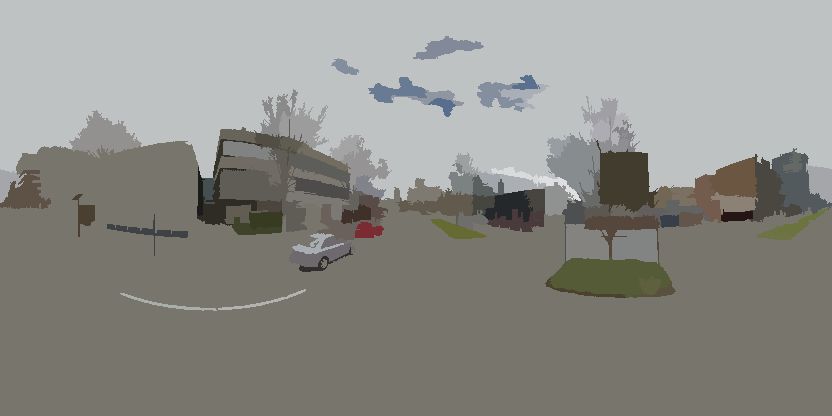
\includegraphics[scale=0.50]{/home/kerryn/git/2018-03-MasterITProject/SkyViewDetection/SkyfinderEvaluationOutput/GSV/mark_output_BigBuilding_5_7.0_210/panorama-ESuX4xmQ_fDc50NK6CnfZQ-1_seg.png} 
c)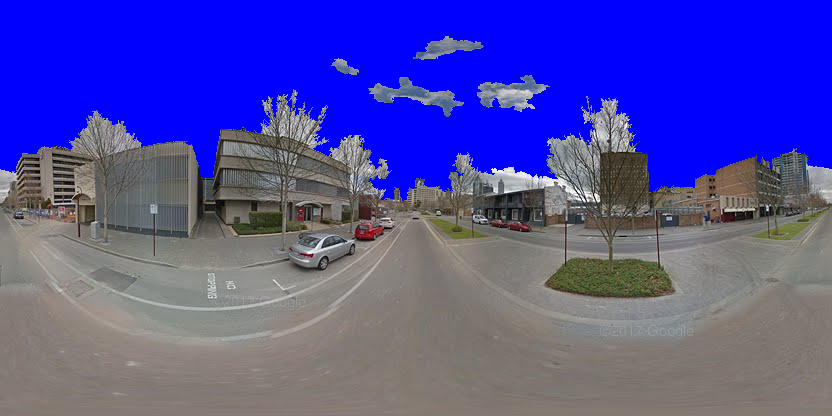
\includegraphics[scale=0.50]{/home/kerryn/git/2018-03-MasterITProject/SkyViewDetection/SkyfinderEvaluationOutput/GSV/mark_output_BigBuilding_5_7.0_210/panorama-ESuX4xmQ_fDc50NK6CnfZQ-1_ms_sky_mark.png} 
\caption{\bf  Results of mean shift (Mean\_5\_7\_210) and HSL filtering, showing a) original image, b) mean shifted image, and c) final marked sky image.}    
 \label{fig:meanresults}  
\end{figure} 



\subsection{K-means clustering and HSL color filtering}\label{sec:kmeans}

K-means clustering was performed using the k-means method from the OpenCV library \citep{Bradski2000}. K-means clustering iteratively splits an image into $K$ number of clusters, terminating when a specified criteria is met (maximum iterations and/or desired accuracy). Three different variations of the input parameters were used, determined experimentally through a sensitivity test to work on a wide variety of images. The technique designations and parameters are detailed in Table \ref{tab:techniques4}. Results shown in Figure \ref{fig:kmeansresults}.


\begin{figure}
\centering    
a)\includegraphics[scale=0.30]{/home/kerryn/git/2018-03-MasterITProject/SkyViewDetection/SkyfinderEvaluationOutput/GSV/mark_output_Cloudy/panorama-ESuX4xmQ_fDc50NK6CnfZQ-1_cropped.png} 
b)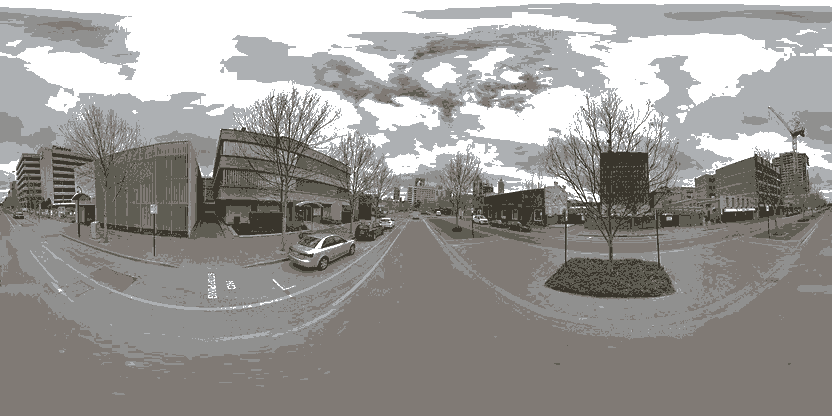
\includegraphics[scale=0.30]{/home/kerryn/git/2018-03-MasterITProject/SkyViewDetection/SkyfinderEvaluationOutput/GSV/mark_output_Cloudy/panorama-ESuX4xmQ_fDc50NK6CnfZQ-1_clustered6.png} 
c)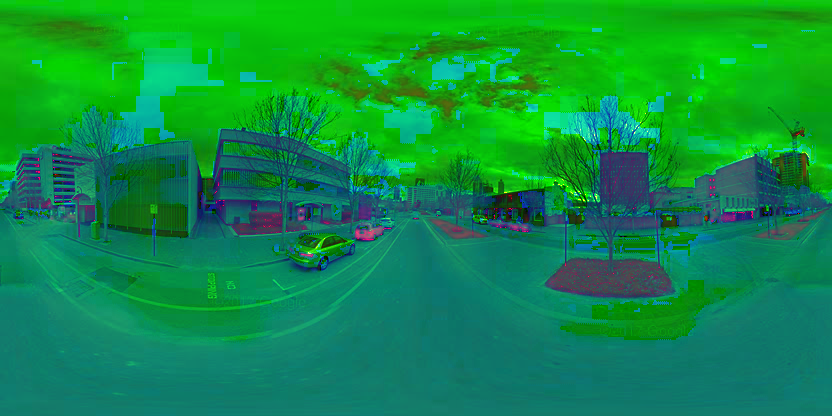
\includegraphics[scale=0.30]{/home/kerryn/git/2018-03-MasterITProject/SkyViewDetection/SkyfinderEvaluationOutput/GSV/mark_output_Cloudy/panorama-ESuX4xmQ_fDc50NK6CnfZQ-1_HLS6.png} 
d)\includegraphics[scale=0.30]{/home/kerryn/git/2018-03-MasterITProject/SkyViewDetection/SkyfinderEvaluationOutput/GSV/mark_output_Cloudy/{panorama-ESuX4xmQ_fDc50NK6CnfZQ-1_sky_mark0.4}.png} 
\caption{\bf  Results of k-means clustering (K-mean\_6) and HSL filtering, showing a) original image, b) k-means clustered image, c) HSL intermediate image, and d) final marked sky image.}    
 \label{fig:kmeansresults}  
\end{figure} 



\subsection{Sobel operator and flood-fill combination}\label{sec:floodfill}

\cite{Middel2018} developed a process based on a Sobel filter and flood-fill algorithm \citep{Sobel1968,Laungrungthip2008,Middel2017}. This method was designed to calculate sky view factor from Google Street View panorama images with the bottom half cropped off and converted to a fisheye projection. \cite{Middel2018} evaluation against 1.6 million locations deep learning classified images reported error rates of RMSE of 0.045 and R$^{2}$ of 0.880.  


\subsection{Inception V3}\label{sec:inception}



\subsection{Neural network training}\label{sec:nntraining}    

The Inception V3 network was used in this study, trained with 300x300 sized imagery. All training and validation images (which consisted of a wide variety of sizes and ratios) were rescaled to 300x300. The network  was calibrated using supervised learning with the generated dataset to identify one of the 13 sky detection techniques and parameters that performed with the highest accuracy for each image. The entire dataset of 38522 images were split into two datasets of 75\% training and 25\% validation. The neural network was trained for 250 epochs on a Nvidia GeForce GTX 1080, requiring about 12 hours. The neural network reached peak accuracy (errs=53.445\%; top5Errs=10.782\%) at epoch 182. To avoid overfitting and overtraining, epoch 182 was used for classification.

%results_per_epoch1:Finished Epoch[182 of 250]: [Validate] ce = 4.20379336 * 9636; errs = 53.445% * 9636; top5Errs = 10.782% * 9636



%Several pre-processing steps were performed before supplying the image to the neural network. Images were randomly cropped from 256x256x3 to Inception V2's native 224x224x3 resolution. No zooming was applied, the aspect ratio was kept fixed, and colour transformations were not used. All images were normalised to [-1, 1] by subtracting a colour value of 128 from each pixel and multiplying by 1/128. To ensure good mixing, training images were randomly allocated to batches. Validation images (25\% of the 1000 training images for each city were reserved as validation data) were transformed to 224x224x3 using central cropping.
%
%
%To update weights in the neural network, a loss function was specified to quantify the extent of any current misclassifications, namely the cross entropy calculated on the softmax layer. Model parameters were calibrated by minimising this loss function using Stochastic Gradient Descent with Nesterov momentum of 0.9. Other parameters included a batch size of 64 samples, reducing learning rate starting at 0.9 per batch, batch normalisation, a dropout rate of 0.2 after the final average-pooling operations, and an L2 regularisation weight per sample of 0.0001. Each model was trained until convergence for a total of 150 epochs, using the Microsoft Cognitive Toolkit (CNTK) \citep{Yu2015}. 
%
%
%\subsection{Neural network inference}\label{sec:methods5}    
%Using the three trained models, inferences were performed using the evaluation datasets for Melbourne and Sydney. As Melbourne and Sydney are not present in the training data, the neural network was forced to choose the city with the most similar characteristics for each of the sampled locations. Using these predictions, every location in both cities was determined to be `most like' another world city from the list due to  characteristics contained within the street map, satellite, or street-view image. Note, all neural network classification predictions with a probability lower than 50\% were filtered out of the following results.

\section{Results}\label{sec:results}




%\begin{figure}
%\centering    
%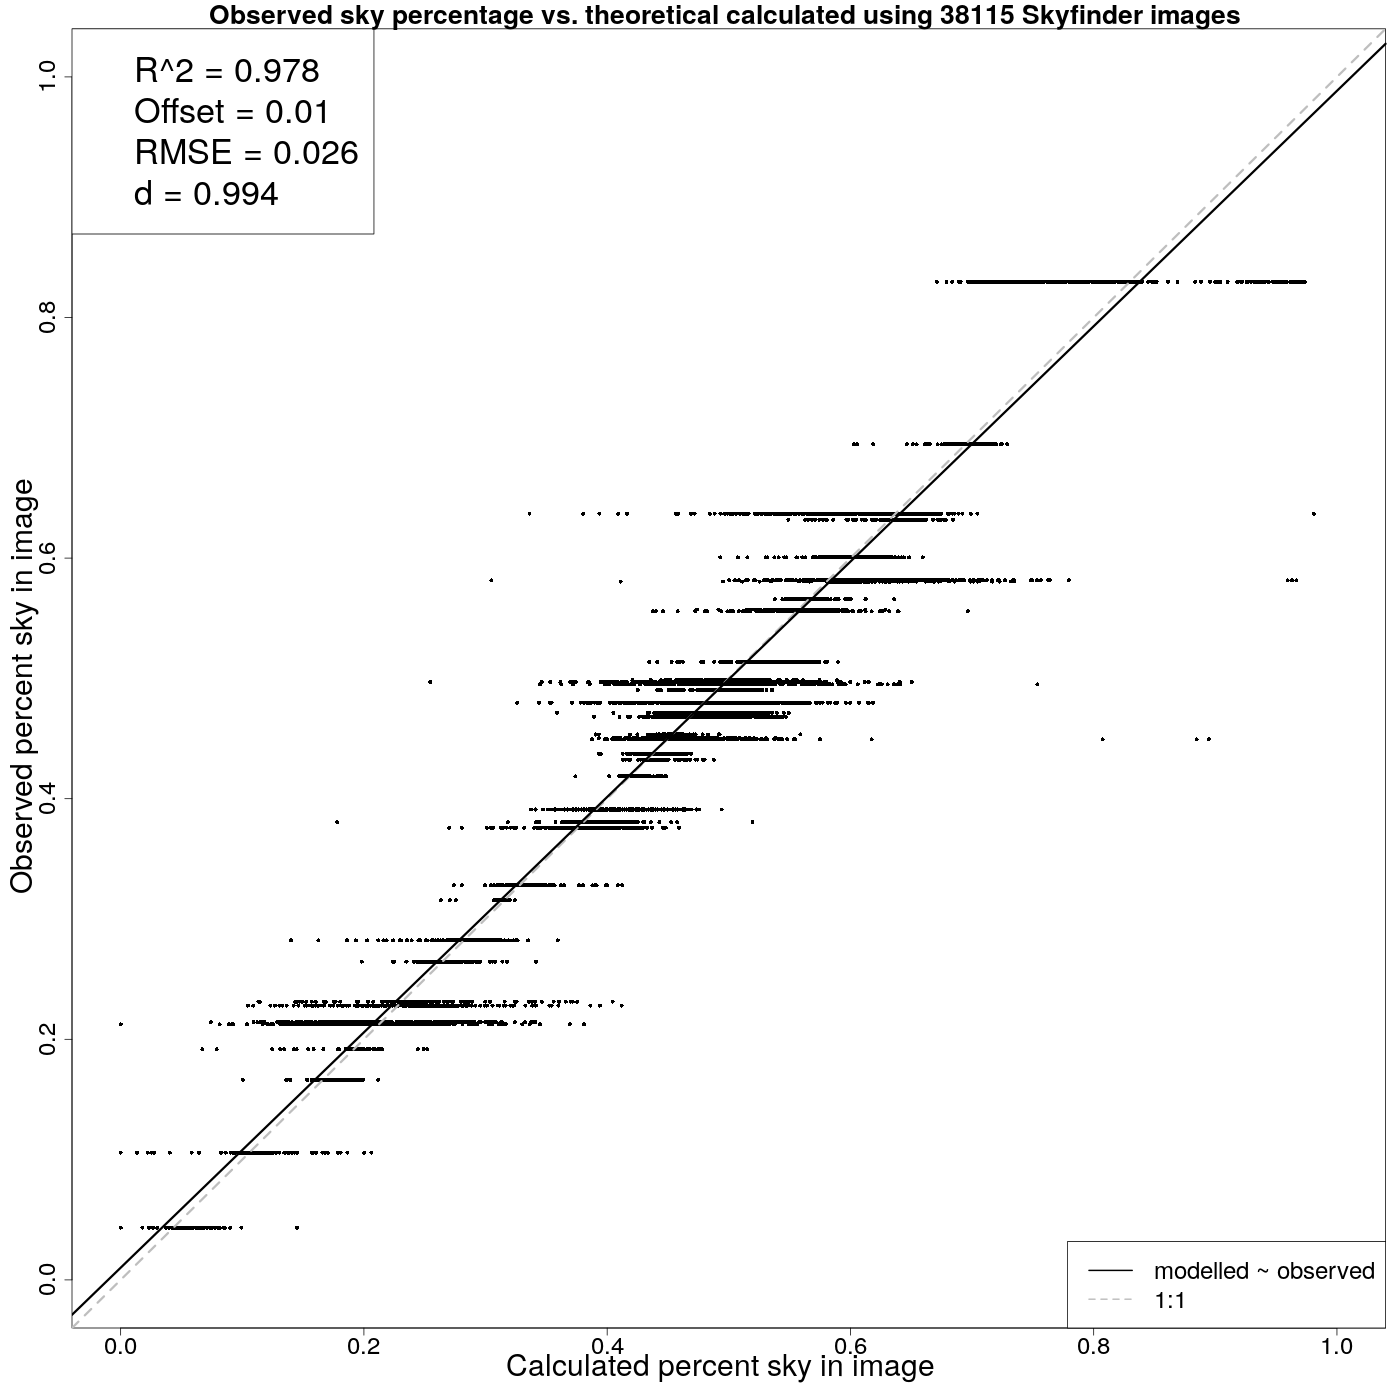
\includegraphics[scale=0.20]{/home/kerryn/git/2018-03-MasterITProject/SkyViewDetection/SkyfinderEvaluationOutput/Plots/ErrorPlots.png}  
%\caption{\bf  XX }    
% \label{fig:mel23000}  
%\end{figure} 

\begin{figure}
\centering
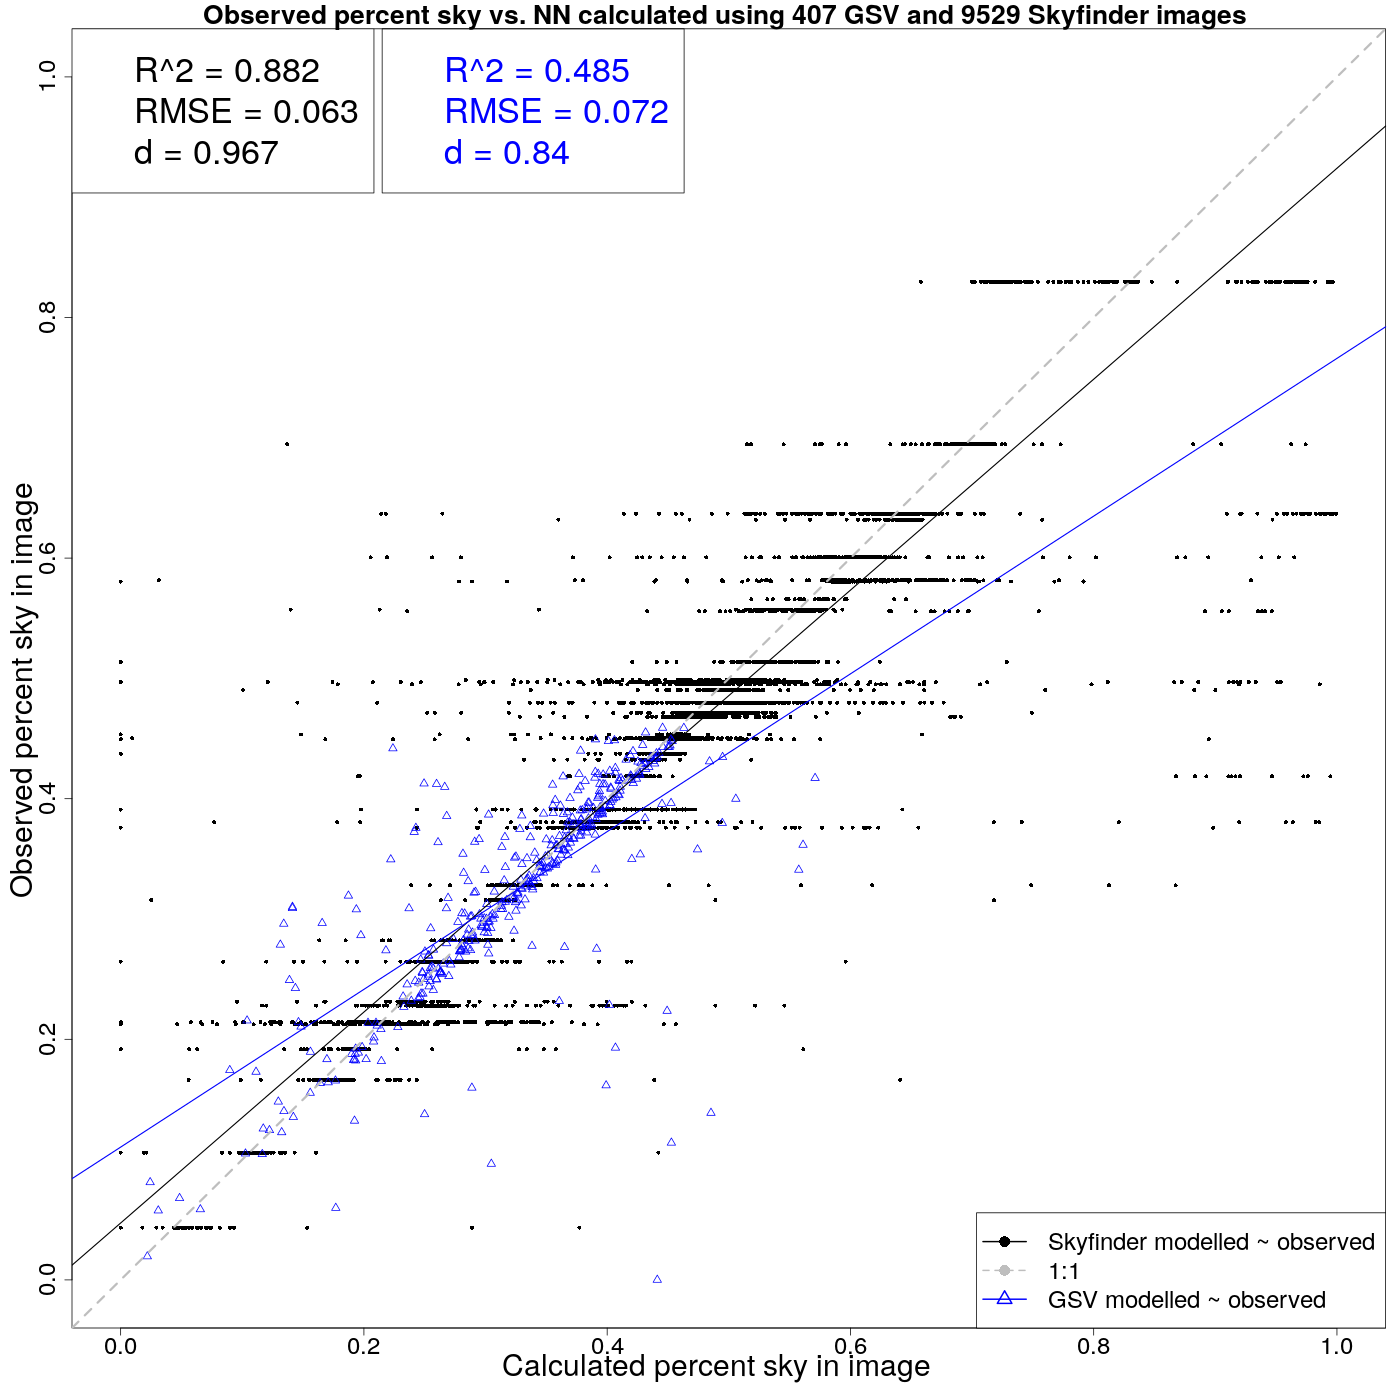
\includegraphics[width=0.7\linewidth]{../2018-03-MasterITProject/SkyViewDetection/SkyfinderEvaluationOutput/Plots/ErrorPlotsCNTK}
\caption{}
\label{fig:errorplotscntk}
\end{figure}

\begin{figure}
\centering
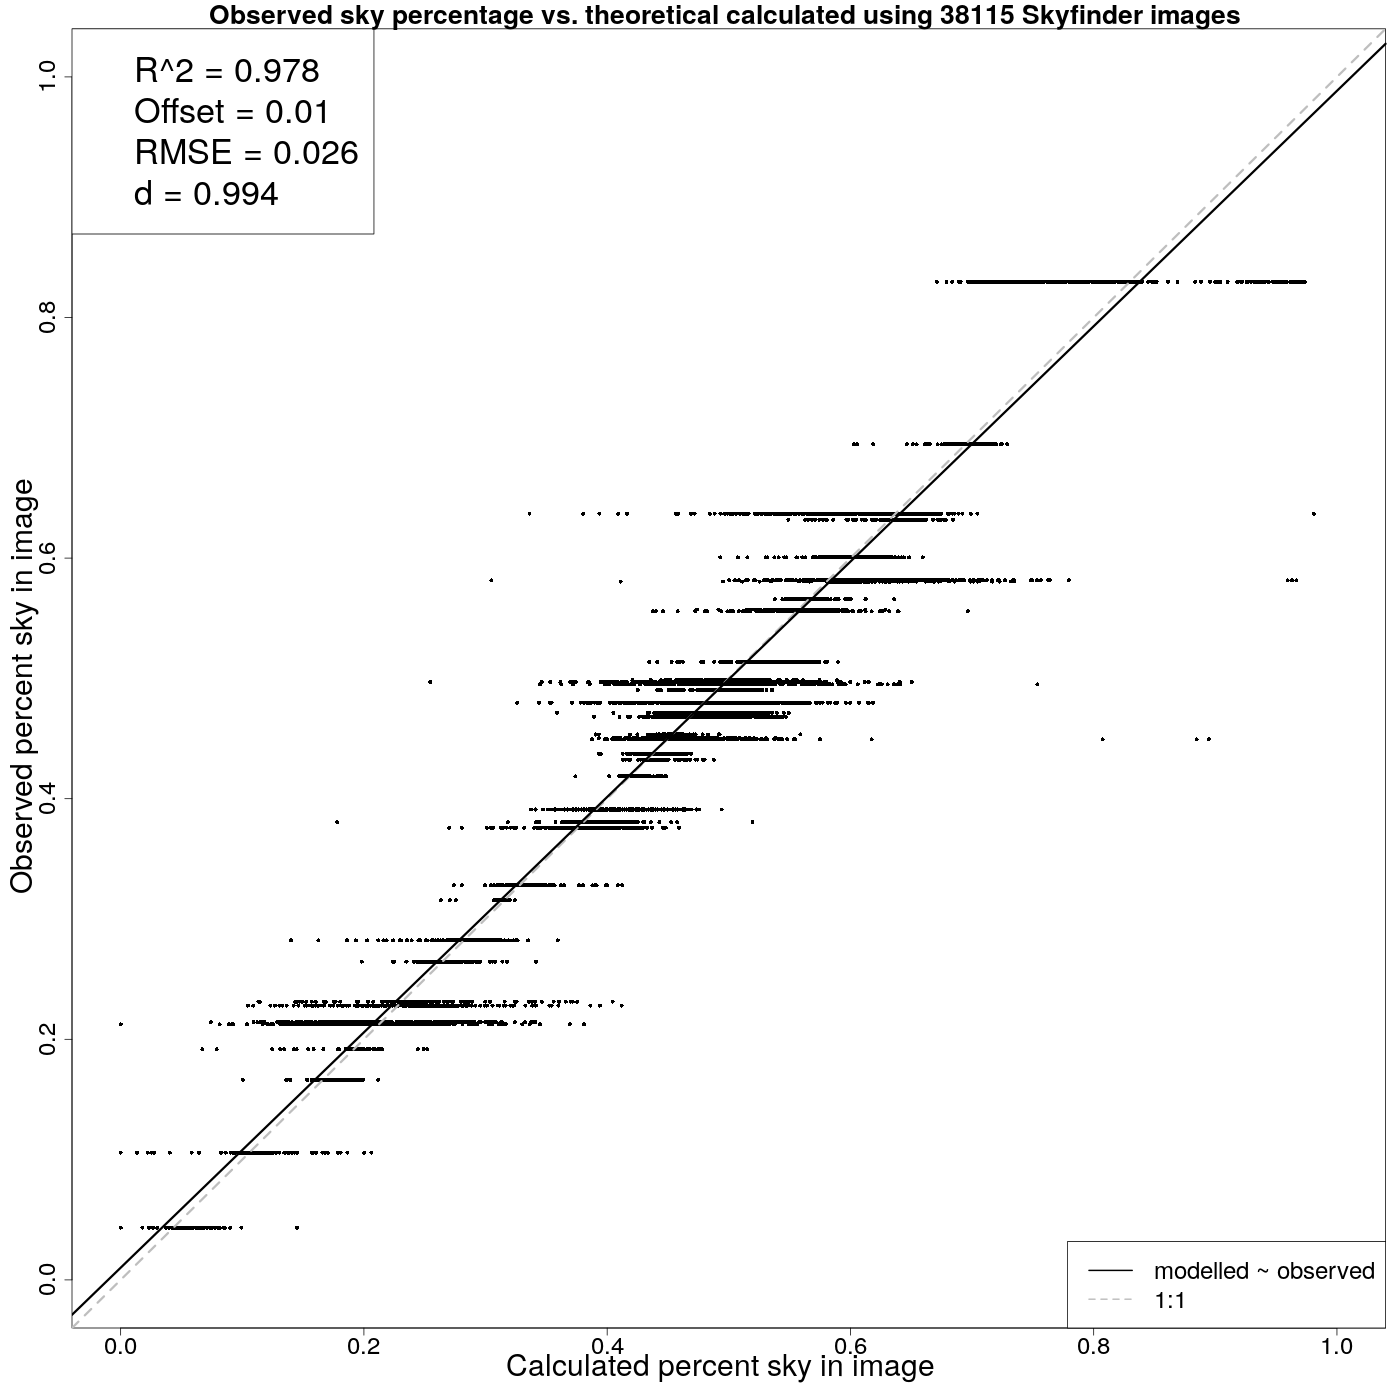
\includegraphics[width=0.7\linewidth]{/home/kerryn/git/2018-03-MasterITProject/SkyViewDetection/SkyfinderEvaluationOutput/Plots/ErrorPlots}
\caption{}
\label{fig:errorplots}
\end{figure}
\begin{figure}
\centering
\includegraphics[width=0.7\linewidth]{/home/kerryn/git/2018-03-MasterITProject/SkyViewDetection/SkyfinderEvaluationOutput/Plots/ErrorPlots1All}
\caption{}
\label{fig:errorplots1all}
\end{figure}
\begin{figure}
\centering
\includegraphics[width=0.7\linewidth]{/home/kerryn/git/2018-03-MasterITProject/SkyViewDetection/SkyfinderEvaluationOutput/Plots/ErrorPlots1K-mean_6}
\caption{}
\label{fig:errorplots1k-mean6}
\end{figure}
\begin{figure}
\centering
\includegraphics[width=0.7\linewidth]{/home/kerryn/git/2018-03-MasterITProject/SkyViewDetection/SkyfinderEvaluationOutput/Plots/ErrorPlots1K-mean_12}
\caption{}
\label{fig:errorplots1k-mean12}
\end{figure}
\begin{figure}
\centering
\includegraphics[width=0.7\linewidth]{/home/kerryn/git/2018-03-MasterITProject/SkyViewDetection/SkyfinderEvaluationOutput/Plots/ErrorPlots1K-mean_14}
\caption{}
\label{fig:errorplots1k-mean14}
\end{figure}
\begin{figure}
\centering
\includegraphics[width=0.7\linewidth]{/home/kerryn/git/2018-03-MasterITProject/SkyViewDetection/SkyfinderEvaluationOutput/Plots/ErrorPlots1Mean_3_6_100}
\caption{}
\label{fig:errorplots1mean36100}
\end{figure}
\begin{figure}
\centering
\includegraphics[width=0.7\linewidth]{/home/kerryn/git/2018-03-MasterITProject/SkyViewDetection/SkyfinderEvaluationOutput/Plots/ErrorPlots1Mean_5_7_210}
\caption{}
\label{fig:errorplots1mean57210}
\end{figure}
\begin{figure}
\centering
\includegraphics[width=0.7\linewidth]{/home/kerryn/git/2018-03-MasterITProject/SkyViewDetection/SkyfinderEvaluationOutput/Plots/ErrorPlots1Mean_7_6_100}
\caption{}
\label{fig:errorplots1mean76100}
\end{figure}
\begin{figure}
\centering
\includegraphics[width=0.7\linewidth]{/home/kerryn/git/2018-03-MasterITProject/SkyViewDetection/SkyfinderEvaluationOutput/Plots/ErrorPlots1Mean_7_8_300}
\caption{}
\label{fig:errorplots1mean78300}
\end{figure}
\begin{figure}
\centering
\includegraphics[width=0.7\linewidth]{/home/kerryn/git/2018-03-MasterITProject/SkyViewDetection/SkyfinderEvaluationOutput/Plots/ErrorPlots1Sobel_50}
\caption{}
\label{fig:errorplots1sobel50}
\end{figure}
\begin{figure}
\centering
\includegraphics[width=0.7\linewidth]{/home/kerryn/git/2018-03-MasterITProject/SkyViewDetection/SkyfinderEvaluationOutput/Plots/ErrorPlots1Sobel_60}
\caption{}
\label{fig:errorplots1sobel60}
\end{figure}
\begin{figure}
\centering
\includegraphics[width=0.7\linewidth]{/home/kerryn/git/2018-03-MasterITProject/SkyViewDetection/SkyfinderEvaluationOutput/Plots/ErrorPlots1Sobel_70}
\caption{}
\label{fig:errorplots1sobel70}
\end{figure}
\begin{figure}
\centering
\includegraphics[width=0.7\linewidth]{/home/kerryn/git/2018-03-MasterITProject/SkyViewDetection/SkyfinderEvaluationOutput/Plots/ErrorPlots1Sobel_80}
\caption{}
\label{fig:errorplots1sobel80}
\end{figure}
\begin{figure}
\centering
\includegraphics[width=0.7\linewidth]{/home/kerryn/git/2018-03-MasterITProject/SkyViewDetection/SkyfinderEvaluationOutput/Plots/ErrorPlots1Sobel_90}
\caption{}
\label{fig:errorplots1sobel90}
\end{figure}
\begin{figure}
\centering
\includegraphics[width=0.7\linewidth]{/home/kerryn/git/2018-03-MasterITProject/SkyViewDetection/SkyfinderEvaluationOutput/Plots/ErrorPlots1Sobel_95}
\caption{}
\label{fig:errorplots1sobel95}
\end{figure}
\begin{figure}
\centering
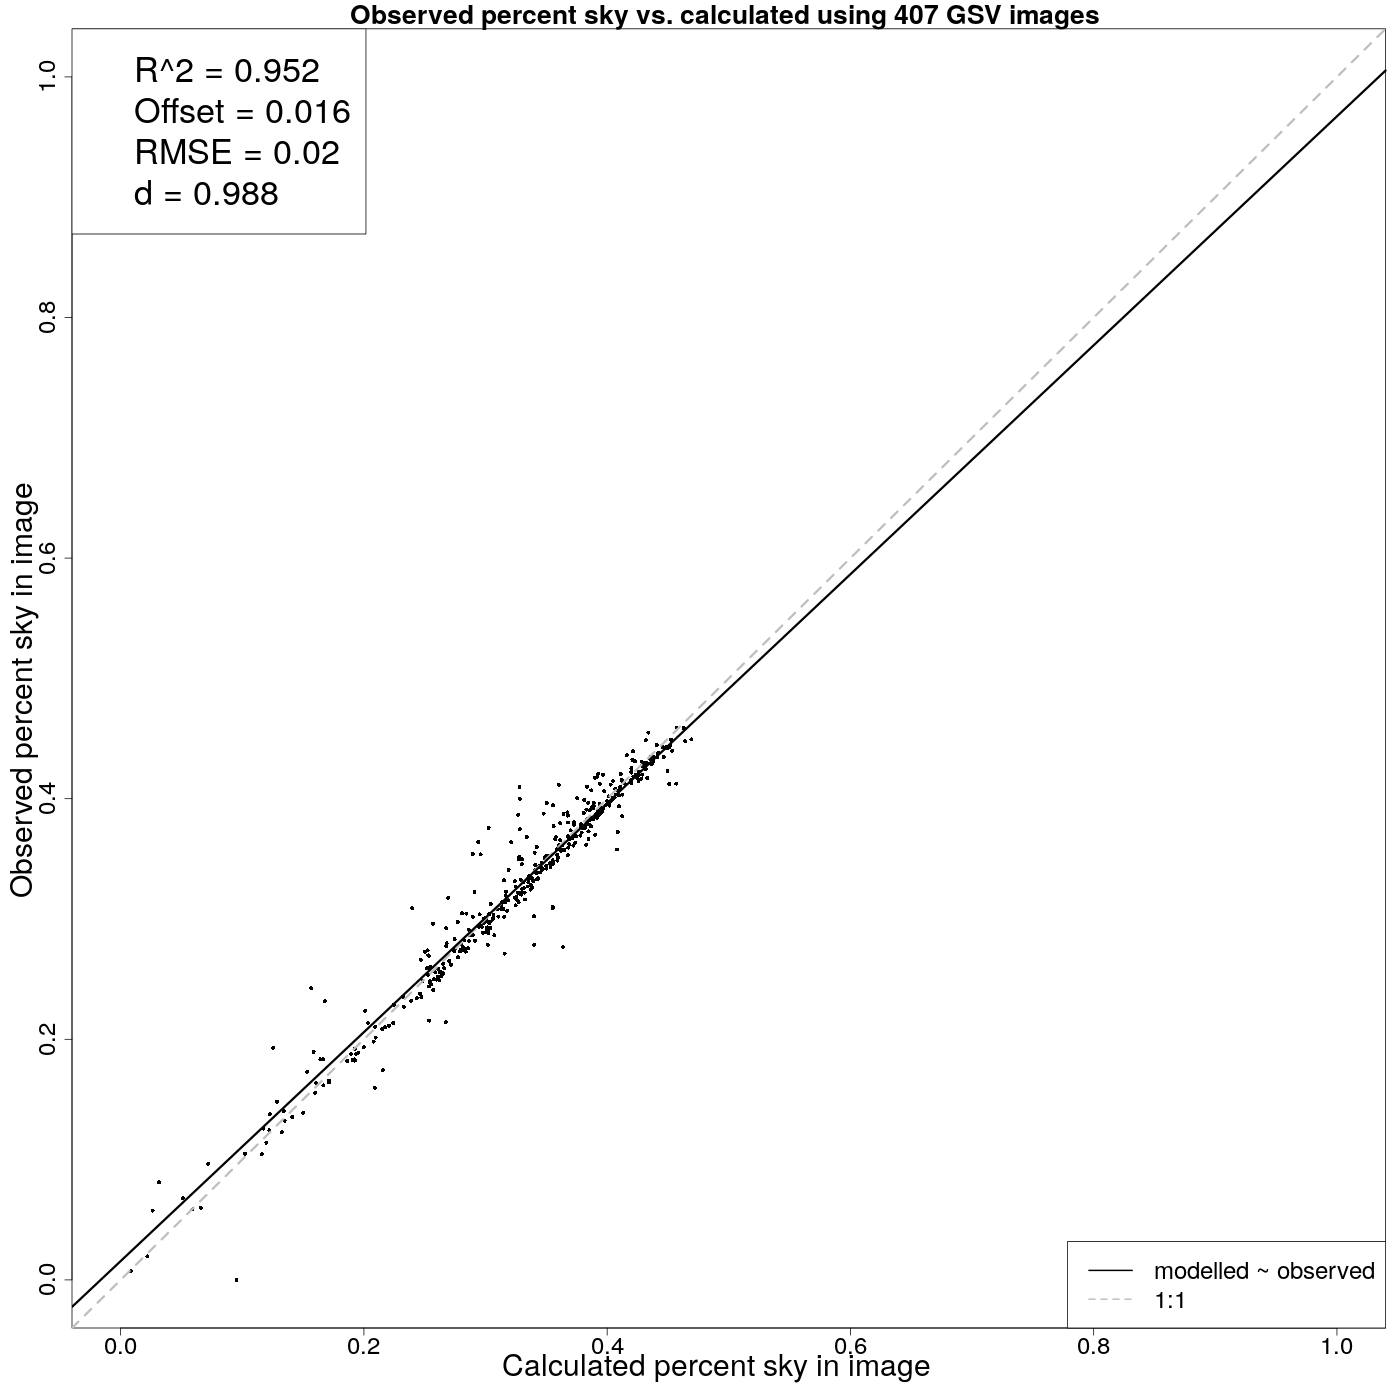
\includegraphics[width=0.7\linewidth]{/home/kerryn/git/2018-03-MasterITProject/SkyViewDetection/SkyfinderEvaluationOutput/Plots/ErrorPlots2}
\caption{}
\label{fig:errorplots2}
\end{figure}
\begin{figure}
\centering
\includegraphics[width=0.7\linewidth]{/home/kerryn/git/2018-03-MasterITProject/SkyViewDetection/SkyfinderEvaluationOutput/Plots/ErrorPlots2All}
\caption{}
\label{fig:errorplots2all}
\end{figure}
\begin{figure}
\centering
\includegraphics[width=0.7\linewidth]{/home/kerryn/git/2018-03-MasterITProject/SkyViewDetection/SkyfinderEvaluationOutput/Plots/ErrorPlots2K-mean_6}
\caption{}
\label{fig:errorplots2k-mean6}
\end{figure}
\begin{figure}
\centering
\includegraphics[width=0.7\linewidth]{/home/kerryn/git/2018-03-MasterITProject/SkyViewDetection/SkyfinderEvaluationOutput/Plots/ErrorPlots2K-mean_12}
\caption{}
\label{fig:errorplots2k-mean12}
\end{figure}
\begin{figure}
\centering
\includegraphics[width=0.7\linewidth]{/home/kerryn/git/2018-03-MasterITProject/SkyViewDetection/SkyfinderEvaluationOutput/Plots/ErrorPlots2K-mean_14}
\caption{}
\label{fig:errorplots2k-mean14}
\end{figure}
\begin{figure}
\centering
\includegraphics[width=0.7\linewidth]{/home/kerryn/git/2018-03-MasterITProject/SkyViewDetection/SkyfinderEvaluationOutput/Plots/ErrorPlots2Mean_3_6_100}
\caption{}
\label{fig:errorplots2mean36100}
\end{figure}
\begin{figure}
\centering
\includegraphics[width=0.7\linewidth]{/home/kerryn/git/2018-03-MasterITProject/SkyViewDetection/SkyfinderEvaluationOutput/Plots/ErrorPlots2Mean_5_7_210}
\caption{}
\label{fig:errorplots2mean57210}
\end{figure}
\begin{figure}
\centering
\includegraphics[width=0.7\linewidth]{/home/kerryn/git/2018-03-MasterITProject/SkyViewDetection/SkyfinderEvaluationOutput/Plots/ErrorPlots2Mean_7_6_100}
\caption{}
\label{fig:errorplots2mean76100}
\end{figure}
\begin{figure}
\centering
\includegraphics[width=0.7\linewidth]{/home/kerryn/git/2018-03-MasterITProject/SkyViewDetection/SkyfinderEvaluationOutput/Plots/ErrorPlots2Mean_7_8_300}
\caption{}
\label{fig:errorplots2mean78300}
\end{figure}
\begin{figure}
\centering
\includegraphics[width=0.7\linewidth]{/home/kerryn/git/2018-03-MasterITProject/SkyViewDetection/SkyfinderEvaluationOutput/Plots/ErrorPlots2Sobel_50}
\caption{}
\label{fig:errorplots2sobel50}
\end{figure}
\begin{figure}
\centering
\includegraphics[width=0.7\linewidth]{/home/kerryn/git/2018-03-MasterITProject/SkyViewDetection/SkyfinderEvaluationOutput/Plots/ErrorPlots2Sobel_60}
\caption{}
\label{fig:errorplots2sobel60}
\end{figure}
\begin{figure}
\centering
\includegraphics[width=0.7\linewidth]{/home/kerryn/git/2018-03-MasterITProject/SkyViewDetection/SkyfinderEvaluationOutput/Plots/ErrorPlots2Sobel_70}
\caption{}
\label{fig:errorplots2sobel70}
\end{figure}
\begin{figure}
\centering
\includegraphics[width=0.7\linewidth]{/home/kerryn/git/2018-03-MasterITProject/SkyViewDetection/SkyfinderEvaluationOutput/Plots/ErrorPlots2Sobel_80}
\caption{}
\label{fig:errorplots2sobel80}
\end{figure}
\begin{figure}
\centering
\includegraphics[width=0.7\linewidth]{/home/kerryn/git/2018-03-MasterITProject/SkyViewDetection/SkyfinderEvaluationOutput/Plots/ErrorPlots2Sobel_90}
\caption{}
\label{fig:errorplots2sobel90}
\end{figure}
\begin{figure}
\centering
\includegraphics[width=0.7\linewidth]{/home/kerryn/git/2018-03-MasterITProject/SkyViewDetection/SkyfinderEvaluationOutput/Plots/ErrorPlots2Sobel_95}
\caption{}
\label{fig:errorplots2sobel95}
\end{figure}

\begin{figure}
\centering
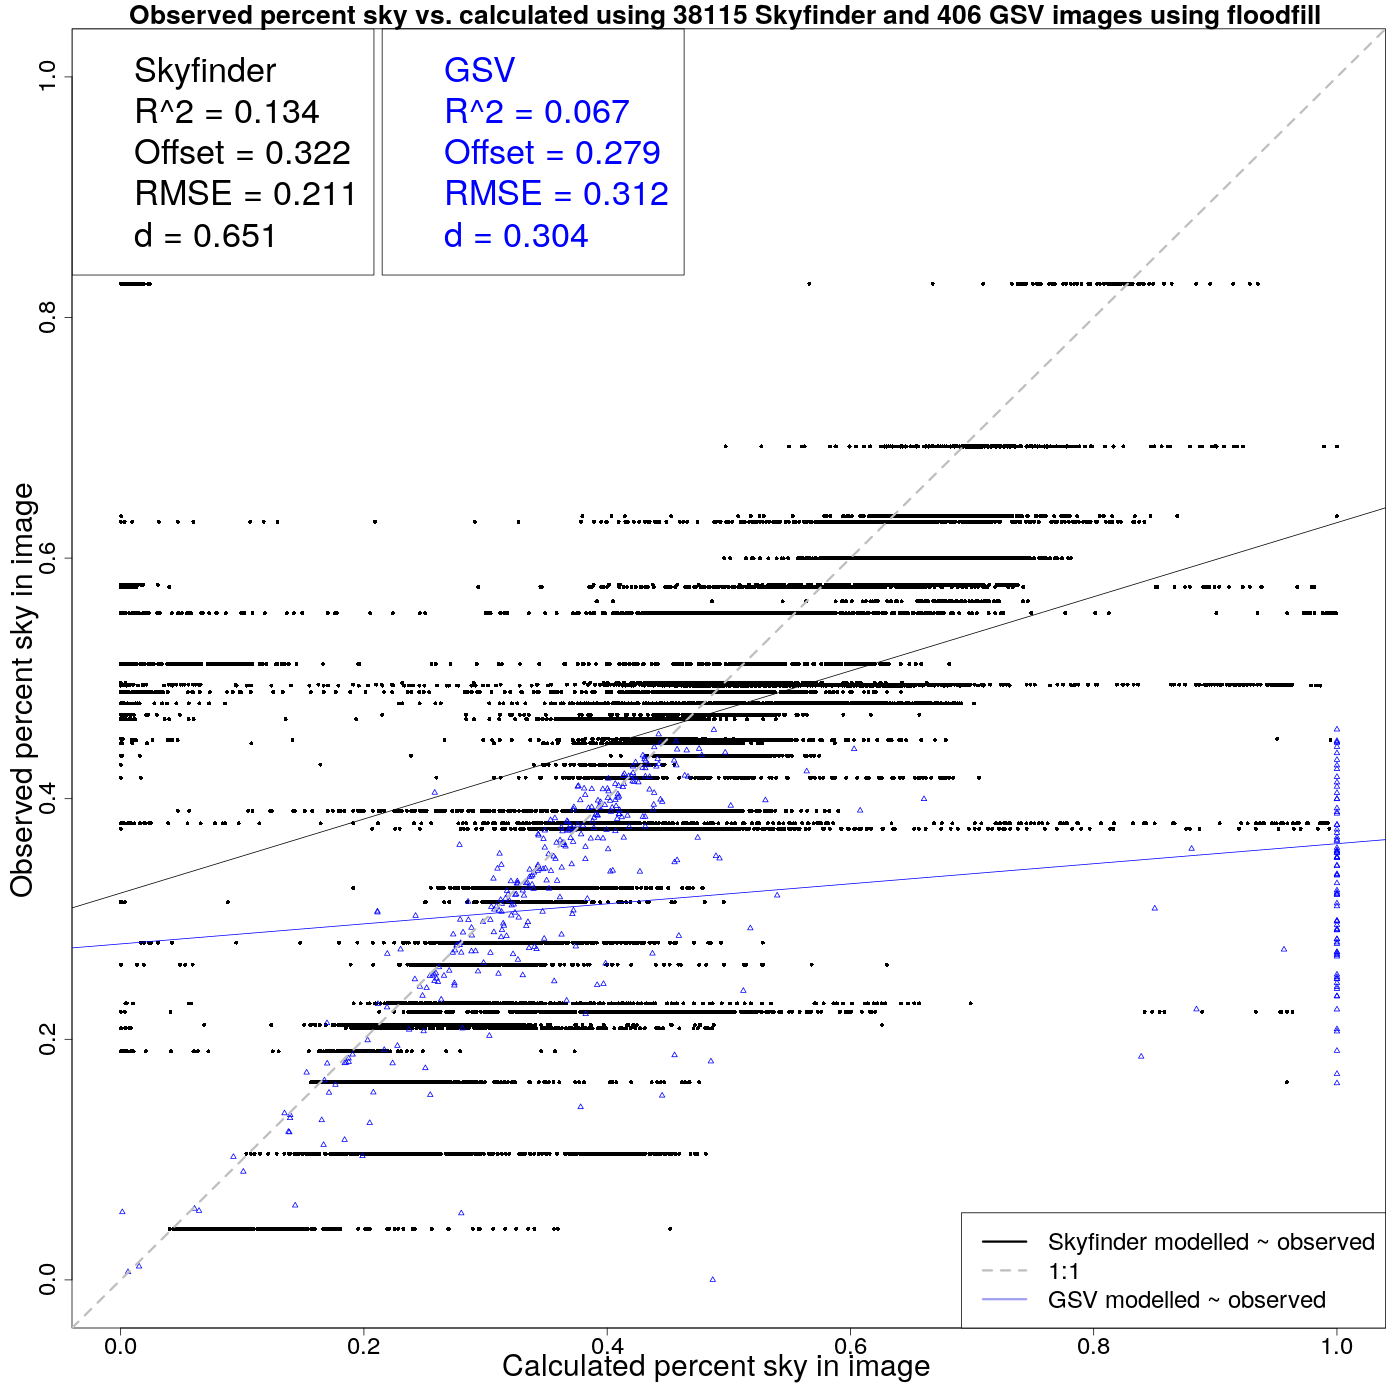
\includegraphics[width=0.7\linewidth]{../2018-03-MasterITProject/SkyViewDetection/SkyfinderEvaluationOutput/Plots/ErrorPlots2FloodfillAll}
\caption{}
\label{fig:errorplots2floodfillall}
\end{figure}




\begin{figure}
\centering
a)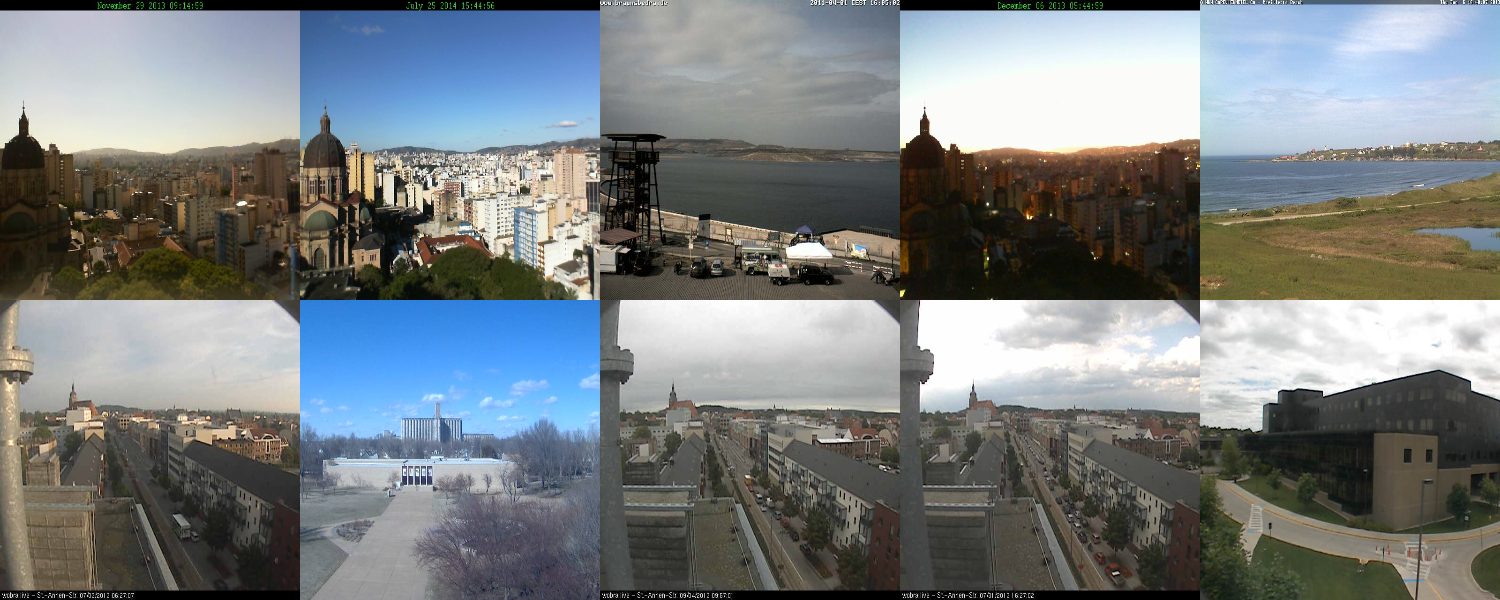
\includegraphics[scale=0.14]{../2018-03-MasterITProject/SkyViewDetection/SkyfinderEvaluationOutput/Plots/13-0_Mean_7_8_300_tiles}
b)\includegraphics[scale=0.14]{../2018-03-MasterITProject/SkyViewDetection/SkyfinderEvaluationOutput/Plots/13-1_Mean_3_6_100_tiles}
c)\includegraphics[scale=0.14]{../2018-03-MasterITProject/SkyViewDetection/SkyfinderEvaluationOutput/Plots/13-2_Mean_5_7_210_tiles}
d)\includegraphics[scale=0.14]{../2018-03-MasterITProject/SkyViewDetection/SkyfinderEvaluationOutput/Plots/13-3_Mean_7_6_100_tiles}
e)\includegraphics[scale=0.14]{../2018-03-MasterITProject/SkyViewDetection/SkyfinderEvaluationOutput/Plots/13-4_K-mean_12_tiles}
f)\includegraphics[scale=0.14]{../2018-03-MasterITProject/SkyViewDetection/SkyfinderEvaluationOutput/Plots/13-5_K-mean_6_tiles}
g)\includegraphics[scale=0.14]{../2018-03-MasterITProject/SkyViewDetection/SkyfinderEvaluationOutput/Plots/13-6_K-mean_14_tiles}
h)\includegraphics[scale=0.14]{../2018-03-MasterITProject/SkyViewDetection/SkyfinderEvaluationOutput/Plots/13-7_Sobel_50_tiles}
i)\includegraphics[scale=0.14]{../2018-03-MasterITProject/SkyViewDetection/SkyfinderEvaluationOutput/Plots/13-8_Sobel_60_tiles}
j)\includegraphics[scale=0.14]{../2018-03-MasterITProject/SkyViewDetection/SkyfinderEvaluationOutput/Plots/13-9_Sobel_70_tiles}
k)\includegraphics[scale=0.14]{../2018-03-MasterITProject/SkyViewDetection/SkyfinderEvaluationOutput/Plots/13-10_Sobel_80_tiles}
l)\includegraphics[scale=0.14]{../2018-03-MasterITProject/SkyViewDetection/SkyfinderEvaluationOutput/Plots/13-11_Sobel_90_tiles}
m)\includegraphics[trim = 0mm 107mm 321mm 0mm, clip,scale=0.14]{../2018-03-MasterITProject/SkyViewDetection/SkyfinderEvaluationOutput/Plots/13-12_Sobel_95_tiles}

\caption{}
\label{fig:13-9_Sobel_70_tiles}
\end{figure}










\section{Conclusion}\label{sec:conclusion}


\section{Code availability and licensing}\label{sec:available}

%TARGET is distributed under the Creative Commons Attribution-NonCommercial-ShareAlike 4.0 Generic (CC BY-NC-SA 4.0). TARGET code cannot be used for commercial purposes. It is available in two versions, Python or Java. The Python code can be downloaded from https://doi.org/10.5281/zenodo.1300023 or Java code is available at  https://zenodo.org/record/1310138. We recommend using the Java version as it runs faster than the Python code. 



%\printglossary[title={List of Symbols}]

\section*{Acknowledgements}
The support of the Commonwealth of Australia through the Cooperative Research Centre program is acknowledged. At Monash University, Kerry Nice was funded by the Cooperative Research Centre for Water Sensitive Cities, an Australian Government initiative. At the University of Melbourne, Kerry Nice was funded by the Transport, Health, and Urban Design (THUD) Hub. 
 
%\end{acknowledgements}

\section*{References}\label{sec:ref}
%% If you have bibdatabase file and want bibtex to generate the
%% bibitems, please use
%%
  \bibliographystyle{elsarticle-harv} 
  \bibliography{library}

%% else use the following coding to input the bibitems directly in the
%% TeX file.

%\begin{thebibliography}{00}
%
%%% \bibitem[Author(year)]{label}
%%% Text of bibliographic item
%
%\bibitem[ ()]{}
%
%\end{thebibliography}


%% The Appendices part is started with the command \appendix;
%% appendix sections are then done as normal sections
%\appendix
%\setcounter{table}{0}
%\renewcommand{\thetable}{A\arabic{table}}

%\subsection{}                               %% Appendix A1, A2, etc.


%%%%%%%%%% taking out parameterizations
%\section{Appendix}\label{sec:app}  
%\subsection{Additional data tables}\label{app:tables}  




%\authorcontribution{This work was developed by Kerry Nice and supervised by Andrew Coutts and Nigel Tapper. Model source code was received from Scott Krayenhoff and Remko Duursma (as acknowledged in Section \ref{sec:available}). Synthesis of this code and new code was developed by Kerry Nice. The article was written by Kerry Nice with editing and suggestions from Andrew Coutts and Nigel Tapper.}
%
%\begin{acknowledgements}
%The work described in this paper was developed during a PhD. project at Monash University. Funding for this was obtailed through the City of Melbourne, Monash University, and the CRC for Water Sensitive Cities.  
%\end{acknowledgements}

%\begin{acknowledgements}
%The support of the Commonwealth of Australia through the Cooperative Research Centre program is acknowledged.
%\end{acknowledgements}






\end{document}

\endinput
%%
%% End of file `elsarticle-template-harv.tex'.
